%======================================================================
\NEWMOD
%======================================================================

\section{\sControl}

%----------------------------------------------------------------------

\logo{\hfill\hyperlink{outline<1>}{\icon}}

\begin{frame}[fragile,label=s-control] 
\modframetitle{\sControl}
\small
\begin{center}
\begin{minipage}{3.25in}
\begin{enumerate}
\item \hyperlink{ss-control<1>}   {\BUTTON {\ssControl}}
\item \hyperlink{ss-adapt<1>}   {\BUTTON {\ssAdapt}}
\item \hyperlink{ss-refresh<1>}   {\BUTTON {\ssRefresh}}
\item \hyperlink{ss-control-summary<1>}   {\BUTTON {\ssControlSummary}}
\end{enumerate}
\end{minipage}
\end{center}
\end{frame}

\logo{\hfill\hyperlink{s-control<1>}{\icon}}

%======================================================================
\NEWSEC
%======================================================================

\subsection{\ssControl}

\begin{frame}[fragile,label=ss-control] 
\secframetitle{\ssControl}

\bluebf{Simulation evolution is controlled in} \bluecode{control\_charm.cpp}

\tikzstyle{decision} = [diamond, draw, fill=blue!20, 
    text width=4.5em, text badly centered, node distance=3cm, inner sep=0pt]
\tikzstyle{block} = [rectangle, draw, fill=blue!20, 
    text width=5em, text centered, rounded corners, minimum height=4em]
\tikzstyle{line} = [draw, -latex']
\tikzstyle{cloud} = [draw, ellipse,fill=red!20, node distance=3cm,
    minimum height=2em]
\ \\
\begin{tikzpicture}[node distance = 3cm, auto]
   \node [block] (init) {Initialize};
   \node [block,below of=init, node distance = 2cm] (adapt) {Adapt};
   \node [block,right of=adapt] (output) {Output};
   \node [block,right of=output] (stopping) {Stopping criteria};
   \node [block,right of=stopping] (compute) {Compute}; 
   \node [block, above of=compute, node distance = 2cm] (refresh) {Refresh};
   \node [coordinate, below of=compute, node distance = 1.5cm] (computenode) {};
   \node [coordinate, below of=adapt, node distance = 1.5cm] (adaptnode) {};

   \path [line] (init) -- (adapt);   
   \path [line] (adapt) -- (output);   
   \path [line] (output) -- (stopping);   
   \path [line] (stopping) -- (compute);   
   \path [line] (compute) -- (refresh);   
   \path [line] (refresh) -- (compute);   
%   \path [line] (compute) -- (adapt);   
 \path [line] (compute.south) -|  (computenode) -- (adaptnode) |- (adapt.south);
\end{tikzpicture}

\end{frame}

 % How are phases of the computation controlled?
%======================================================================
\NEWSEC
%======================================================================

\subsection{\ssAdapt}

%----------------------------------------------------------------------

\begin{frame}[fragile,label=ss-adapt] 
\secframetitle{\ssAdapt}
\bluebf{Mesh refinement proceeds in several steps}

\begin{enumerate}
\item Apply refinement criteria (\code{Refine})
\item Tell neighbor \code{Block}s your desired level
\begin{itemize}
\item \code{Block}s form a chare array
\item remote entry method call to neighbor blocks
\end{itemize}
\item Receive neighbor level
\begin{itemize}
\item entry method
\item called by neighbors
\end{itemize}
\item Update own level if needed (goto \bluebf{2})
\item Exit after \blueit{quiescence}
\begin{itemize}
\item no processor is executing an entry point
\item no messages are awaiting processing
\item and no messages in-flight
\end{itemize}
\end{enumerate}
\end{frame}

%----------------------------------------------------------------------

\begin{frame}[fragile]
\secframetitle{\ssAdapt}
\begin{center}
\begin{minipage}{3in}
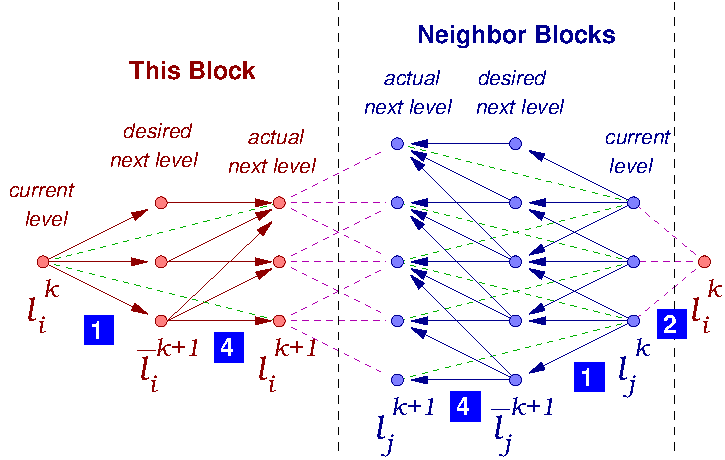
\includegraphics[width=3in]{amr-2.pdf}
\end{minipage}
\end{center}
\pause
\begin{itemize}
\item \greentext{temporal level jump criterion}
\pause
\item \magentatext{spacial level jump criterion}
\end{itemize}
\end{frame}

%----------------------------------------------------------------------

\begin{frame}[fragile] 
\secframetitle{\ssAdapt}
\blockblue
\begin{center}
\begin{minipage}{2.5in}
\ANIMATEGRAPHICS{width=2.5in}{40}{Images/Circle/mesh-00}{475}{951}
\end{minipage}
\end{center}
\end{frame}
 % How does Cello implement AMR?
%======================================================================
\NEWSEC
%======================================================================

\subsection{\ssRefresh}

%----------------------------------------------------------------------

\begin{frame}[fragile,label=ss-refresh] 
\secframetitle{\ssRefresh}
\framesubtitle{Neighbor in same refinement level}
%\blockblue
\begin{minipage}{2.0in}
\begin{center}
   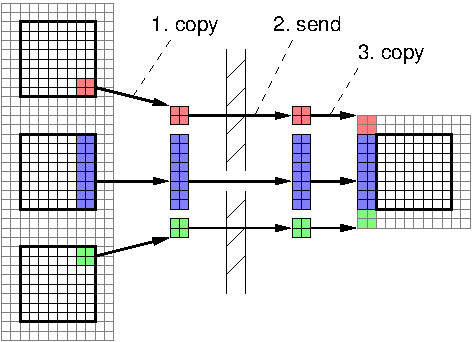
\includegraphics[width=2.0in]{refresh-same.pdf} \ \\
\end{center}
\end{minipage} \ 
\begin{minipage}{2.1in}
\begin{enumerate}
\item Face data copied to array
\begin{itemize}
\item \bluecode{FieldFace} object
\end{itemize}
\item Array sent to neighbor
\begin{itemize}
\item chare entry method
\item array sent as message
\end{itemize}
\item Array copied to ghost zones
\end{enumerate}
\end{minipage}
\vspace{0.2in}
\ \\
\ \\
\bluetext{Refresh ends when arrays from all neighbors have been received.}
\end{frame}

%----------------------------------------------------------------------

\begin{frame}[fragile]
\secframetitle{\ssRefresh}
\framesubtitle{Neighbor in coarser refinement level}
%\blockblue
\begin{minipage}{2.0in}
\begin{center}
   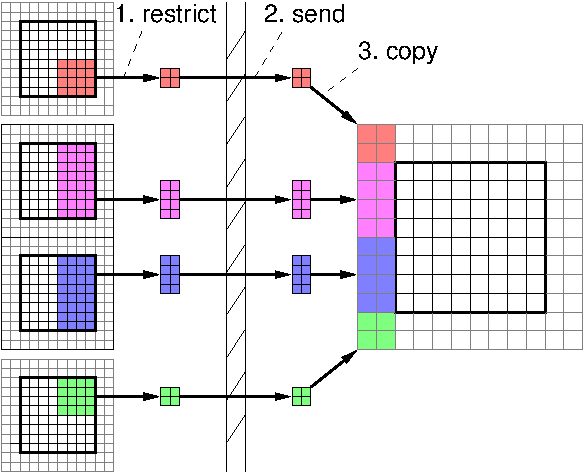
\includegraphics[width=2.0in]{refresh-coarse.pdf} \ \\
\end{center}
\end{minipage} \ 
\begin{minipage}{2.1in}
\begin{enumerate}
\item Face data coarsened to array
\begin{itemize}
\item \code{Restrict} object
\item \code{FieldFace} array
\end{itemize}
\item Array sent to neighbor
\item Array copied to ghost zones
\end{enumerate}
\end{minipage}
\end{frame}

%----------------------------------------------------------------------

\begin{frame}[fragile]
\secframetitle{\ssRefresh}
\framesubtitle{Neighbor in finer refinement level}
%\blockblue
\begin{minipage}{2.0in}
\begin{center}
   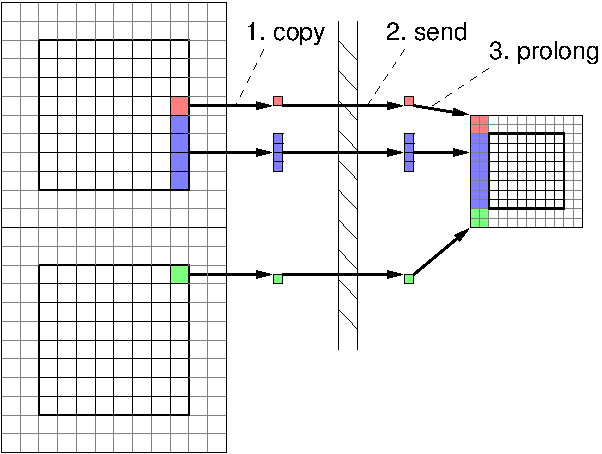
\includegraphics[width=2.0in]{refresh-fine.pdf} \ \\
\end{center}
\end{minipage}
\begin{minipage}{2.1in}
\begin{enumerate}
\item Face data copied to array
\item Array sent to neighbor
\item Data interpolated to ghost zones
\begin{itemize}
\item \code{Prolong} object
\end{itemize}
\end{enumerate}
\end{minipage}
\end{frame}

%----------------------------------------------------------------------

%\secframetitle{\ssRefresh}
%%\blockblue
%\begin{center}
%\begin{tabular}{|c|c|c|} \hline
%\begin{minipage}{1.0in}
%\onslide<1-> \vspace{0.1in} $\boldsymbol{L}$ \textcolor{red}{$\Rightarrow L$} \vspace{0.1in} \hfill  \ \\
%   \includegraphics<1->[height=0.8in]{n-send-same.pdf} \ \\
%\end{minipage} \pause &
%\begin{minipage}{1.0in}
%\onslide<2-> \vspace{0.1in} $\boldsymbol{L}$ \textcolor{red}{$\Rightarrow L-1$} \vspace{0.1in} \hfill  \ \\ 
%   \includegraphics<2->[height=0.8in]{n-send-coarse.pdf} \ \\
%\end{minipage} \pause  &
%\begin{minipage}{1.0in}
%\onslide<3->  \vspace{0.1in} $\boldsymbol{L}$ \textcolor{red}{$\Rightarrow L+1$}\vspace{0.1in} \hfill \ \\ 
%   \includegraphics<3->[height=0.8in]{n-send-fine.pdf} \ \\
%\end{minipage} \pause \\ \hline
%\begin{minipage}{1.0in}
%\onslide<4->  \vspace{0.1in} \hfill \textcolor{blue}{$L \Rightarrow$} $ \boldsymbol{L}$ \vspace{0.1in}  \ \\
%   \includegraphics<4->[height=0.8in]{n-recv-same.pdf} \ \\
%\end{minipage}  &
%\begin{minipage}{1.0in}
%\onslide<5->  \vspace{0.1in} \hfill \textcolor{blue}{$L+1 \Rightarrow$} $ \boldsymbol{L}$\vspace{0.1in}  \ \\
%   \includegraphics<5->[height=0.8in]{n-recv-fine.pdf} \ \\
%\end{minipage}  &
%\begin{minipage}{1.0in}
%\onslide<6->   \vspace{0.1in} \hfill \textcolor{blue}{$L-1 \Rightarrow$} $ \boldsymbol{L}$\vspace{0.1in}  \ \\  
%   \includegraphics<6->[height=0.8in]{n-recv-coarse.pdf} \ \\
%\end{minipage} \\ \hline
%\end{tabular}
%\end{center}
%\end{frame}

 % How does Cello exchange data between blocks?
%======================================================================
\NEWSEC
%======================================================================

\subsection{\ssControlSummary}

%----------------------------------------------------------------------

\begin{frame}[fragile,label=ss-control-summary] 
\secframetitle{\ssControlSummary}

\vfill
\centerline{$\qed$}
\end{frame}

 % How does Cello exchange data between blocks?
